\documentclass[12pt]{article}              
\usepackage[margin=1.5cm]{geometry}
\usepackage{setspace,relsize}               
\usepackage{moreverb}                        
\usepackage{url}
\usepackage{hyperref}
\hypersetup{colorlinks=true,citecolor=blue}
\usepackage{amsmath}
\usepackage{mathtools} 
\usepackage{amssymb}
\usepackage{indentfirst}
\usepackage[authoryear,round]{natbib}
\bibliographystyle{apalike}
\usepackage[pdftex]{lscape}
% \usepackage{float}
% \usepackage{longtable}
% \usetikzlibrary{arrows}
%%%%
\title{
Estimating the Initial Susceptible Fraction in Dengue Dynamics
}           
\author{Flavio Code\c{c}o Coelho \\
School of Applied Mathematics, Get\'ulio Vargas Foundation (FGV) \\
\& \\
Luiz Max de Carvalho \\
Program for Scientific Computing (PROCC), Oswaldo Cruz Foundation}

\date{\today}
% Notation defs
\def \rr {$R_{t}\ $}

\usepackage{Sweave}
\begin{document}                                  
\input{draft_lm1-concordance}

%
\maketitle
\begin{abstract}
We derive confidence/credibility bounds for the uncertainty about the estimate of the effective reproductive number $R_t$ under the assumption that reported disease counts are Poisson distributed.
It is shown that one can construct a conservative confidence interval for \rr using the induced probability distribution that results from the approach of \citet{mantel}.
\end{abstract}
%%%%%%%%%%%%%%%%%%%%%%%%%%%%%%%%%%%%%%%%%%%%%%%%%%%%%
%%%%%%%%%%%%%%%%%%%%%%%%%%%%%%%%%%%%%%%%%%%%%%%%%%%%%
\section{Background}
\label{sec:intro}

In monitoring of infectious diseases, it is important to assess whether the incidence of a a particular disease is increasing significantly, in order to decide to take preventive measures.
The effective reproductive number at time $t$, \rr, can be understood as a real-time estimate of the basic reproductive number ($R_{0}$) and is defined as the average number of secondary cases per primary case at time $t$.
Let $Y_t$ be the number of reported disease cases for a particular time $t \in (0, T)$.
\citet{nishiura} extend the theory developed by \citet{stallybrass} and propose to estimate \rr as
\begin{equation}
\label{eq:Rtestimate}
R_t = \left( \frac{Y_{t+1}}{Y_t}\right)^{1/n}
\end{equation}
where $n$ is taken to be the ratio between the length of reporting interval and the mean generation time of the disease.
Here we are interested in the simpler case $n=1$.
If \rr is to be used as a decision tool, one needs to be able to quantify the uncertainty about estimate in equation~\ref{eq:Rtestimate}. 
Here we detail how to obtain confidence intervals for \rr, exploring two approaches under the assumption that the counts $Y_t$ are Poisson distributed for all $t$.

\newpage
\section{Approaches}

\subsection{Ederer \& Mantel (1974)}
\label{sec:mantel}

First we explore the approach of \citet{mantel}, whose objective is to obtain confidence intervals for the ratio of two Poisson counts. 
Let $Y_{t} \sim Poisson(\lambda_t)$ and $Y_{t+1} \sim Poisson(\lambda_{t+1})$ and define $S = Y_{t} + Y_{t+1}$.
The authors then proceed to note that by conditioning on the sum $S$
\begin{align}
\label{eq:binlike}
Y_{t+1} | S &\sim Binomial(S, \theta_t) \\
\theta_t &= \frac{\lambda_{t+1}}{\lambda_{t} + \lambda_{t+1}}
\end{align}
Let $c_{\alpha}(\theta_t) = \{\theta_t^{(L)} , \theta_t^{(U)} \}$ be such that $Pr(\theta_t^{(L)}<\theta_t <\theta_t^{(U)}) = \alpha$.
Analogously, define $c_{\alpha}(R_t) = \{R_t^{(L)} , R_t^{(U)} \}$ such that $Pr(R_t^{(L)}<R_t<R_t^{(U)}) = \alpha$.
\citet{mantel} show that one can construct a $100\alpha \%$ confidence interval for \rr by noting that
\begin{align}
 R_t^{(L)} &= \frac{\theta_t^{(L)}}{(1-\theta_t^{(L)})}\\
 R_t^{(U)} &= \frac{\theta_t^{(U)}}{(1-\theta_t^{(U)})}
\end{align}

Many authors have derived $c_{\alpha}(\theta_t)$ following orthodox approaches such as those of \citet{wilson} and \citet{clopper}, mainly for simplicity reasons.
We choose instead to take a Bayesian approach and use the  $100\alpha \%$ posterior credibility interval for $\theta_t$ as $c_{\alpha}(\theta_t)$.
If we choose the conjugate beta prior with parameters $a_0$ and $b_0$ for the binomial likelihood in (\ref{eq:binlike}), the posterior distribution for $\theta_t$ is
\begin{equation}
\label{eq:thetapost}
p(\theta_t| Y_{t+1}, S) \sim Beta(Y_{t+1} + a_0, Y_t + b_0)
\end{equation}
Equation~(\ref{eq:thetapost}) tells us that the induced distribution of $R_t$ is a beta prime with parameters $ a_1 = Y_{t+1} + a_0$ and $b_1 =  Y_t + b_0$.
The density of this induced distribution  $f_P(R_t)$ is then 
\begin{equation}
\label{eq:densityMantel}
f_P(R_t| a_1, b_1) = \frac{\Gamma(a_1 + b_1)}{\Gamma(a_1)\Gamma(b_1)} R_t^{a_1 - 1} (1 + R_t)^{-(a_1 + b_1)}
\end{equation}
Thus, the expectation of \rr under $f_P$ is $a_1/(b_1 - 1)$ and its variance is $a_1(a_1 + b_1 - 1)/\left((b_1 - 2)(b_1 - 1)^2 \right) $.

Since when $R_t > 1$ indicates sustained transmission, one may be interested in computing the probability of this event.
By noting that
\begin{align}
\label{cumprobMantel}
Pr(R_t > 1) &= 1 - \int_0^1 f_P(r)dr \\
            &= 1- Pr(\theta_t < \frac{1}{2})
\end{align}
one can avoid dealing with the density in~(\ref{eq:densityMantel}) directly.

% \subsection{Nishiura et al. (2010)}
% \label{sec:nishiura}
% 
% An alternative approach is to use the conditional distribution of \rr on $Y_{t+1}$ and $Y_t$ as defined in equation A7 of \citet{nishiura}:
% \begin{equation}
% \label{eq:unorm}
% f_{R}(R_{t}) = (Y_tR_{t})^{Y_{t+1}} e^{-Y_tR_{t}}
% \end{equation}
% Noticing the kernel of (\ref{eq:unorm}) is that of a gamma distribution with $a_2 = Y_{t+1}+1$ and $b_2 = Y_t$, we obtain a proper density from which to construct $c_{\alpha}(R_t)$, simply by computing the appropriate quantiles of said distribution.
%  This density is
% \begin{equation}
% \label{eq:densityNishiura}
% f_N(R_t| a_2, b_2) =  \frac{b_2^{a_2}}{\Gamma(a_2)} R_t^{a_2-1} e^{-b_2 R_t}
% \end{equation}
% Once again $Pr(R_t>1)$ can be easily computed using
% \begin{equation}
% \label{eq:cdfNishiura}
% P(R_t > 1) = 1-F_N(1) = 1- \frac{1}{\Gamma(a_2)} \gamma(a_2, b_2)
% \end{equation}
% where $F_N(R_t)$ is the distribution function of $R_t$ and $\gamma(\cdot)$ is the incomplete gamma function.

\subsection{A remark on prior distributions and tail behaviour}
\label{sec:tails}

In order to decide which approach to take, it may be of use analysing the variance and tail behaviour of the derived distributions for \rr. 
Consider the case of using a flat $Uniform(0, 1)$ prior for $\theta_t$ in Section~\ref{sec:mantel}.
With $a_0 = b_0 = 1$, $a_1 = a_2$ and $b_1 = b_2 + 1$.
The beta prime (inverse beta distribution) will have heavier tails compared to the conditional distribution in (\ref{eq:densityNishiura}), thus providing more conservative confidence/credibility intervals.  
As a side note, the Bayesian approach presented in Section~\ref{sec:mantel} will give similar results to those of \citet{wilson} and \citet{wilson} for $Y_{t+1}$ and $Y_t >> 1$.
Under the flat  uniform prior for $\theta_t$, the Bayesian posterior credibility interval is nearly indistinguishable from the confidence interval proposed by \citet{clopper} for $Y_{t+1}, Y_t > 20$.
Note that the $Beta(1, 1)$ uniform prior for $\theta_t$ constitutes a poor prior choice mainly because the induced distribution for \rr is only well-defined for $b_0 > 2$.

The main advange of the Bayesian approach is that one can devise prior distributions for $\theta_t$ taking advantage of the intuitive parametrisation and flexibility of the beta family of distributions.
Prior elicitation can also be done for \rr and the hyperparameters directly plugged into the prior for $\theta_t$. 
One can, for example, choose a priori mean and variance for \rr and find $a_0$ and $b_0$ that satisfy those conditions.
Let $m_0$ and $v_0$ be the prior expectation and variance for $R_t$. 
After some tedious algebra one finds
\begin{align}
\label{eq:elicitation}
a_0 &= \frac{m_0v_0 + m_0^3 + m_0^2}{v_0} \\
b_0 &= \frac{2v_0 + m_0^2 + m_0}{v_0}
\end{align}
If one wants only to specify $m_0$ and a coefficient of variation $c$ \footnote{$c = \sqrt{v_0}/ m_0$.} for $R_t$ \textit{a priori}, some less boring algebra gives:
\begin{align}
\label{eq:elicitationcv}
a_0 &= \frac{m_0^3c^2 + m_0^3 + m_0^2}{m_0^2c^2} \\
b_0 &= \frac{2m_0^2c^2 + m^2 + m}{m_0^2c^2}
\end{align}

\newpage
\section{Preliminary results -- Dengue notifications in Rio de Janeiro}
\label{sec:dataanalysis}

We now show the application of the methods described above to dengue notification data in the city of Rio de Janeiro.
The data consists of weekly dengue notifications for 10 Health Planning Areas (APS, in Portuguese) for the period 2010-2014.
Figure~\ref{fig:casesperAPS} shows the data.
We compute $c_{\alpha}(R_t)$ for the total (sum) number of notifications using the two approaches described, using a generation time of $3$ weeks and choose $a_0$ and $b_0$ such that $E[R_t] = 1/2$ and $Var(R_t) = 2$.
The resulting estimates and $95\%$ confidence bounds are presented in Figure~\ref{fig:confidencetotals}.
Finally, we compute $Pr(R_t > 1)$ using the two distributions discussed here (Figure~\ref{fig:pRt1}).

\section{Final Remarks}
\label{sec:remarks}

Both strategies presented here seem appropriate to the quantification of uncertainty about $R_t$.
The distribution obtained by combining the approach of \citet{mantel} with Bayesian inference for $\theta_t$, however, possesses heavier tails and thus offers more conservative bounds.
Additionally, the ability to specify prior information on $R_t$ based on expert knowledge may prove useful.


\section{Acknowlegements}
LMC is grateful to Dr. Leonardo Bastos for useful discussions.
\newpage
%%%%%%%%%%%%%%%%%%%%%%%%%%%%%%%%%%%%%%%%%%%%%%%%%%%%%%%%%%%%
\begin{figure}[!h]
\setkeys{Gin}{scale=.7}
\begin{center}
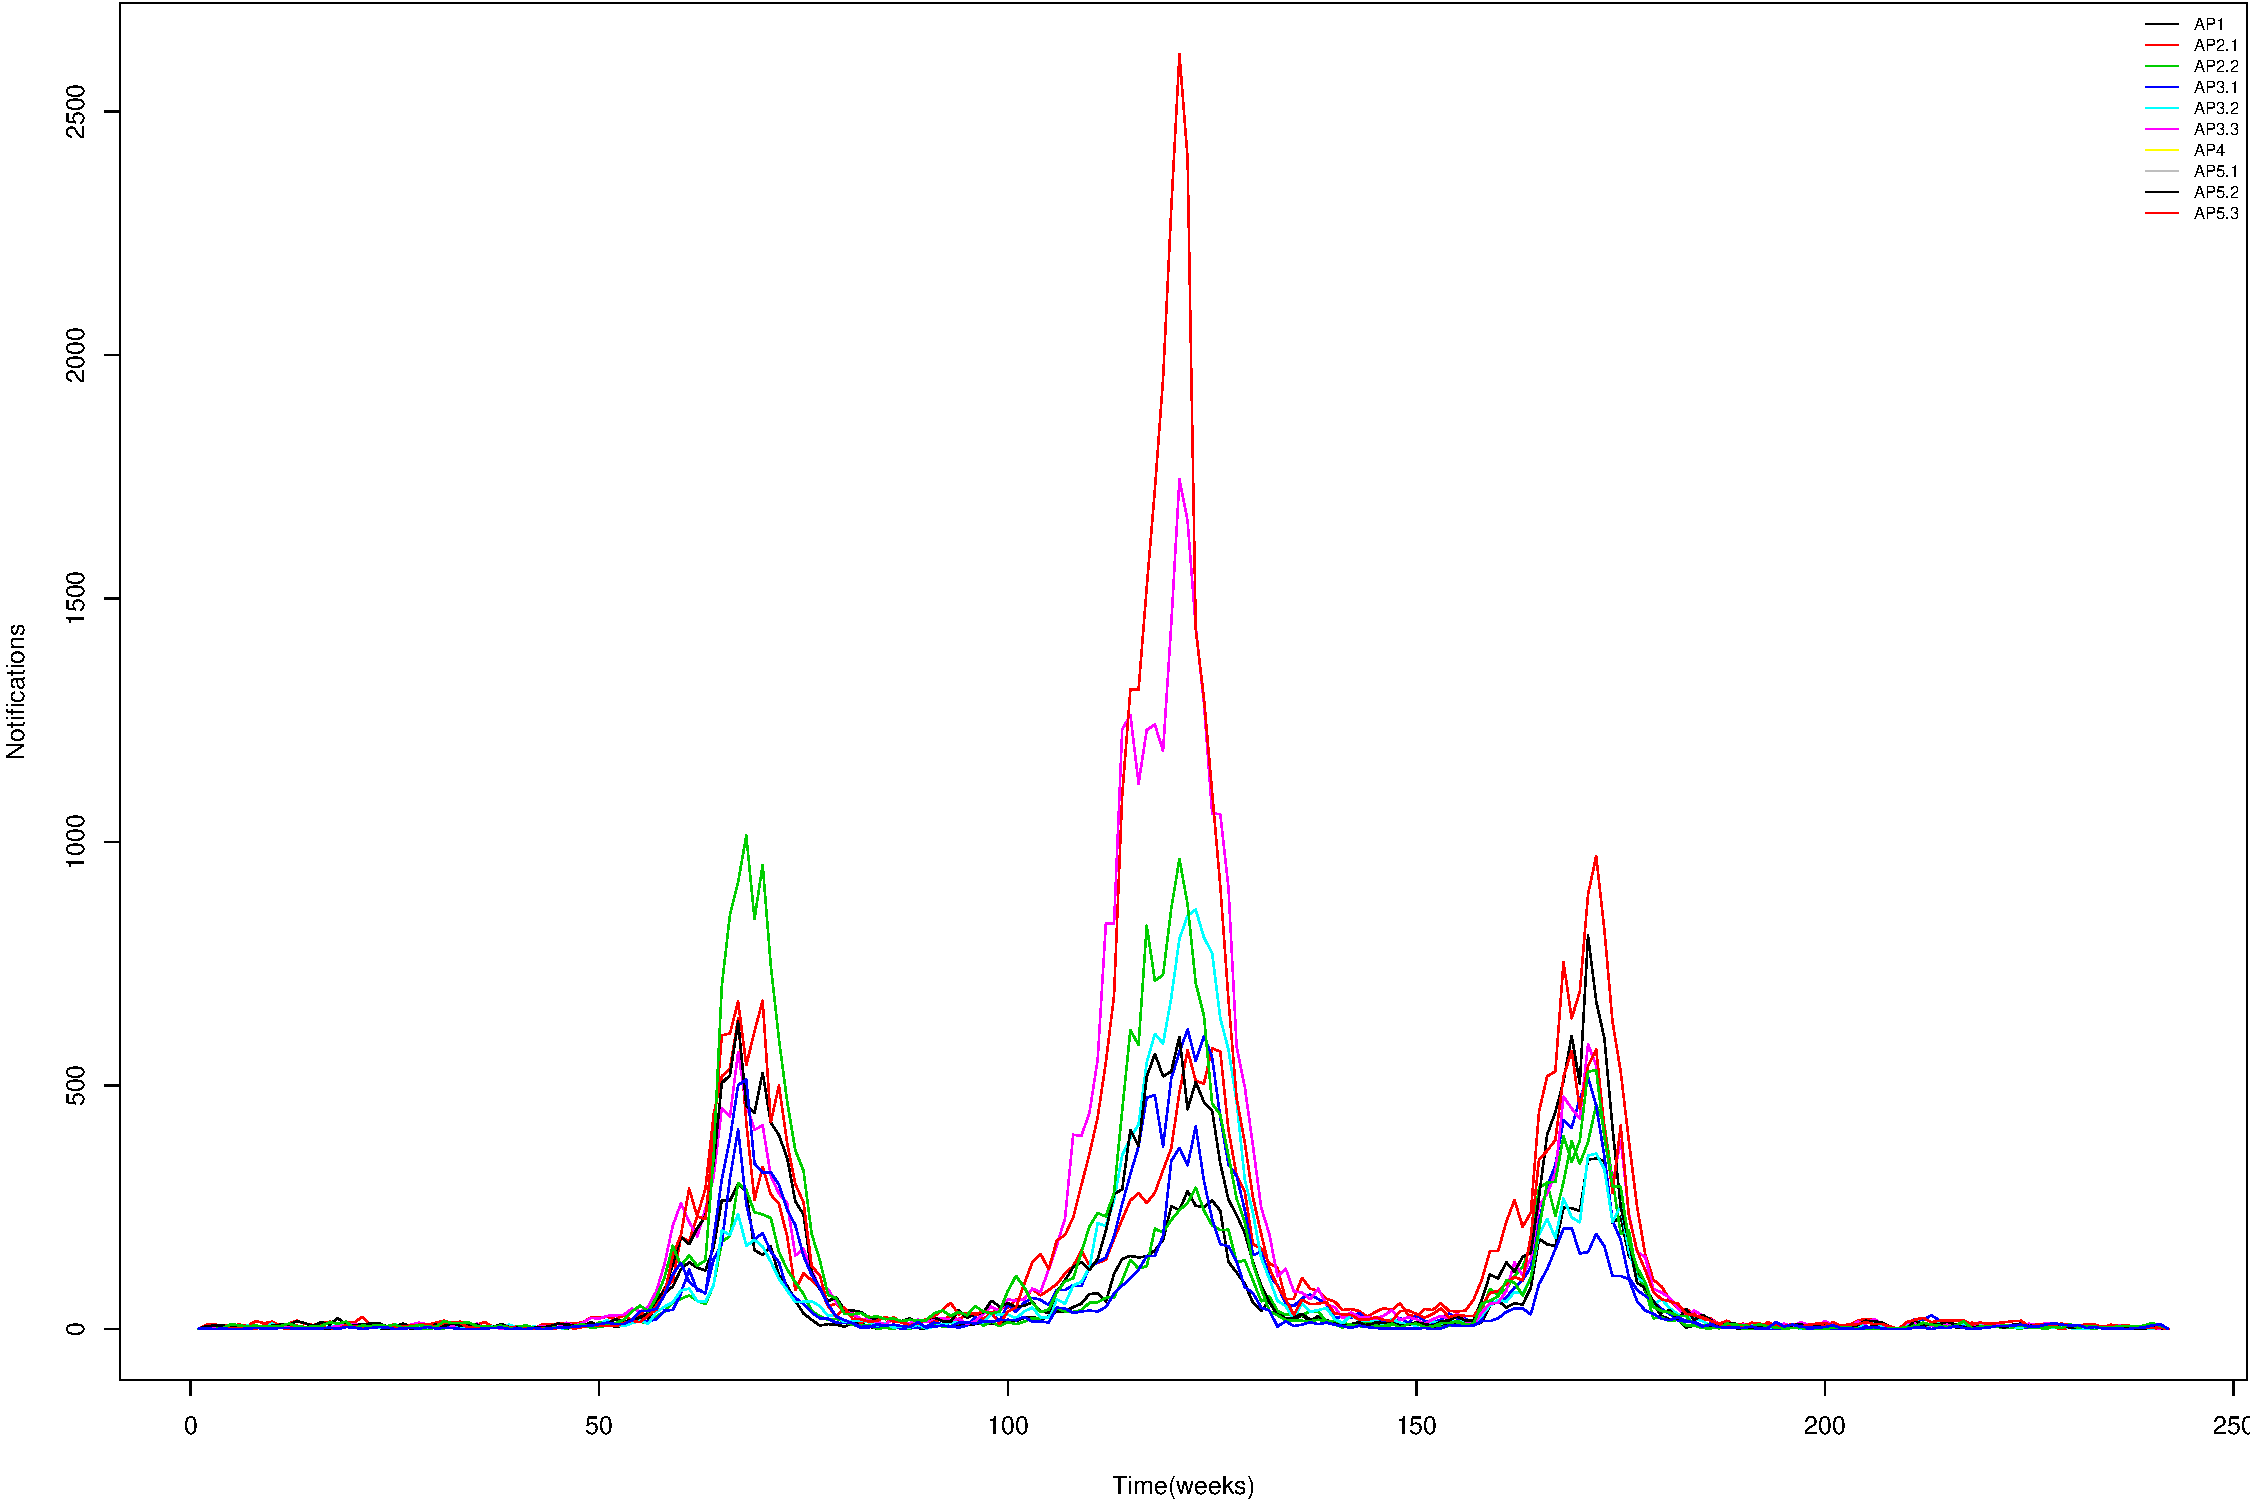
\includegraphics{FIGURES/figure-002}
\end{center}
\caption{Total number of dengue notifications per HPA (APS)}
\label{fig:casesperAPS}
\end{figure}
%%%%%%%%%%%%%%%%%%%%%%%%%%%%%%%%%%%%%%%%%%%%%%%%%%%%%%%%%
\begin{figure}[!h]
\setkeys{Gin}{scale=.7}
\begin{center}
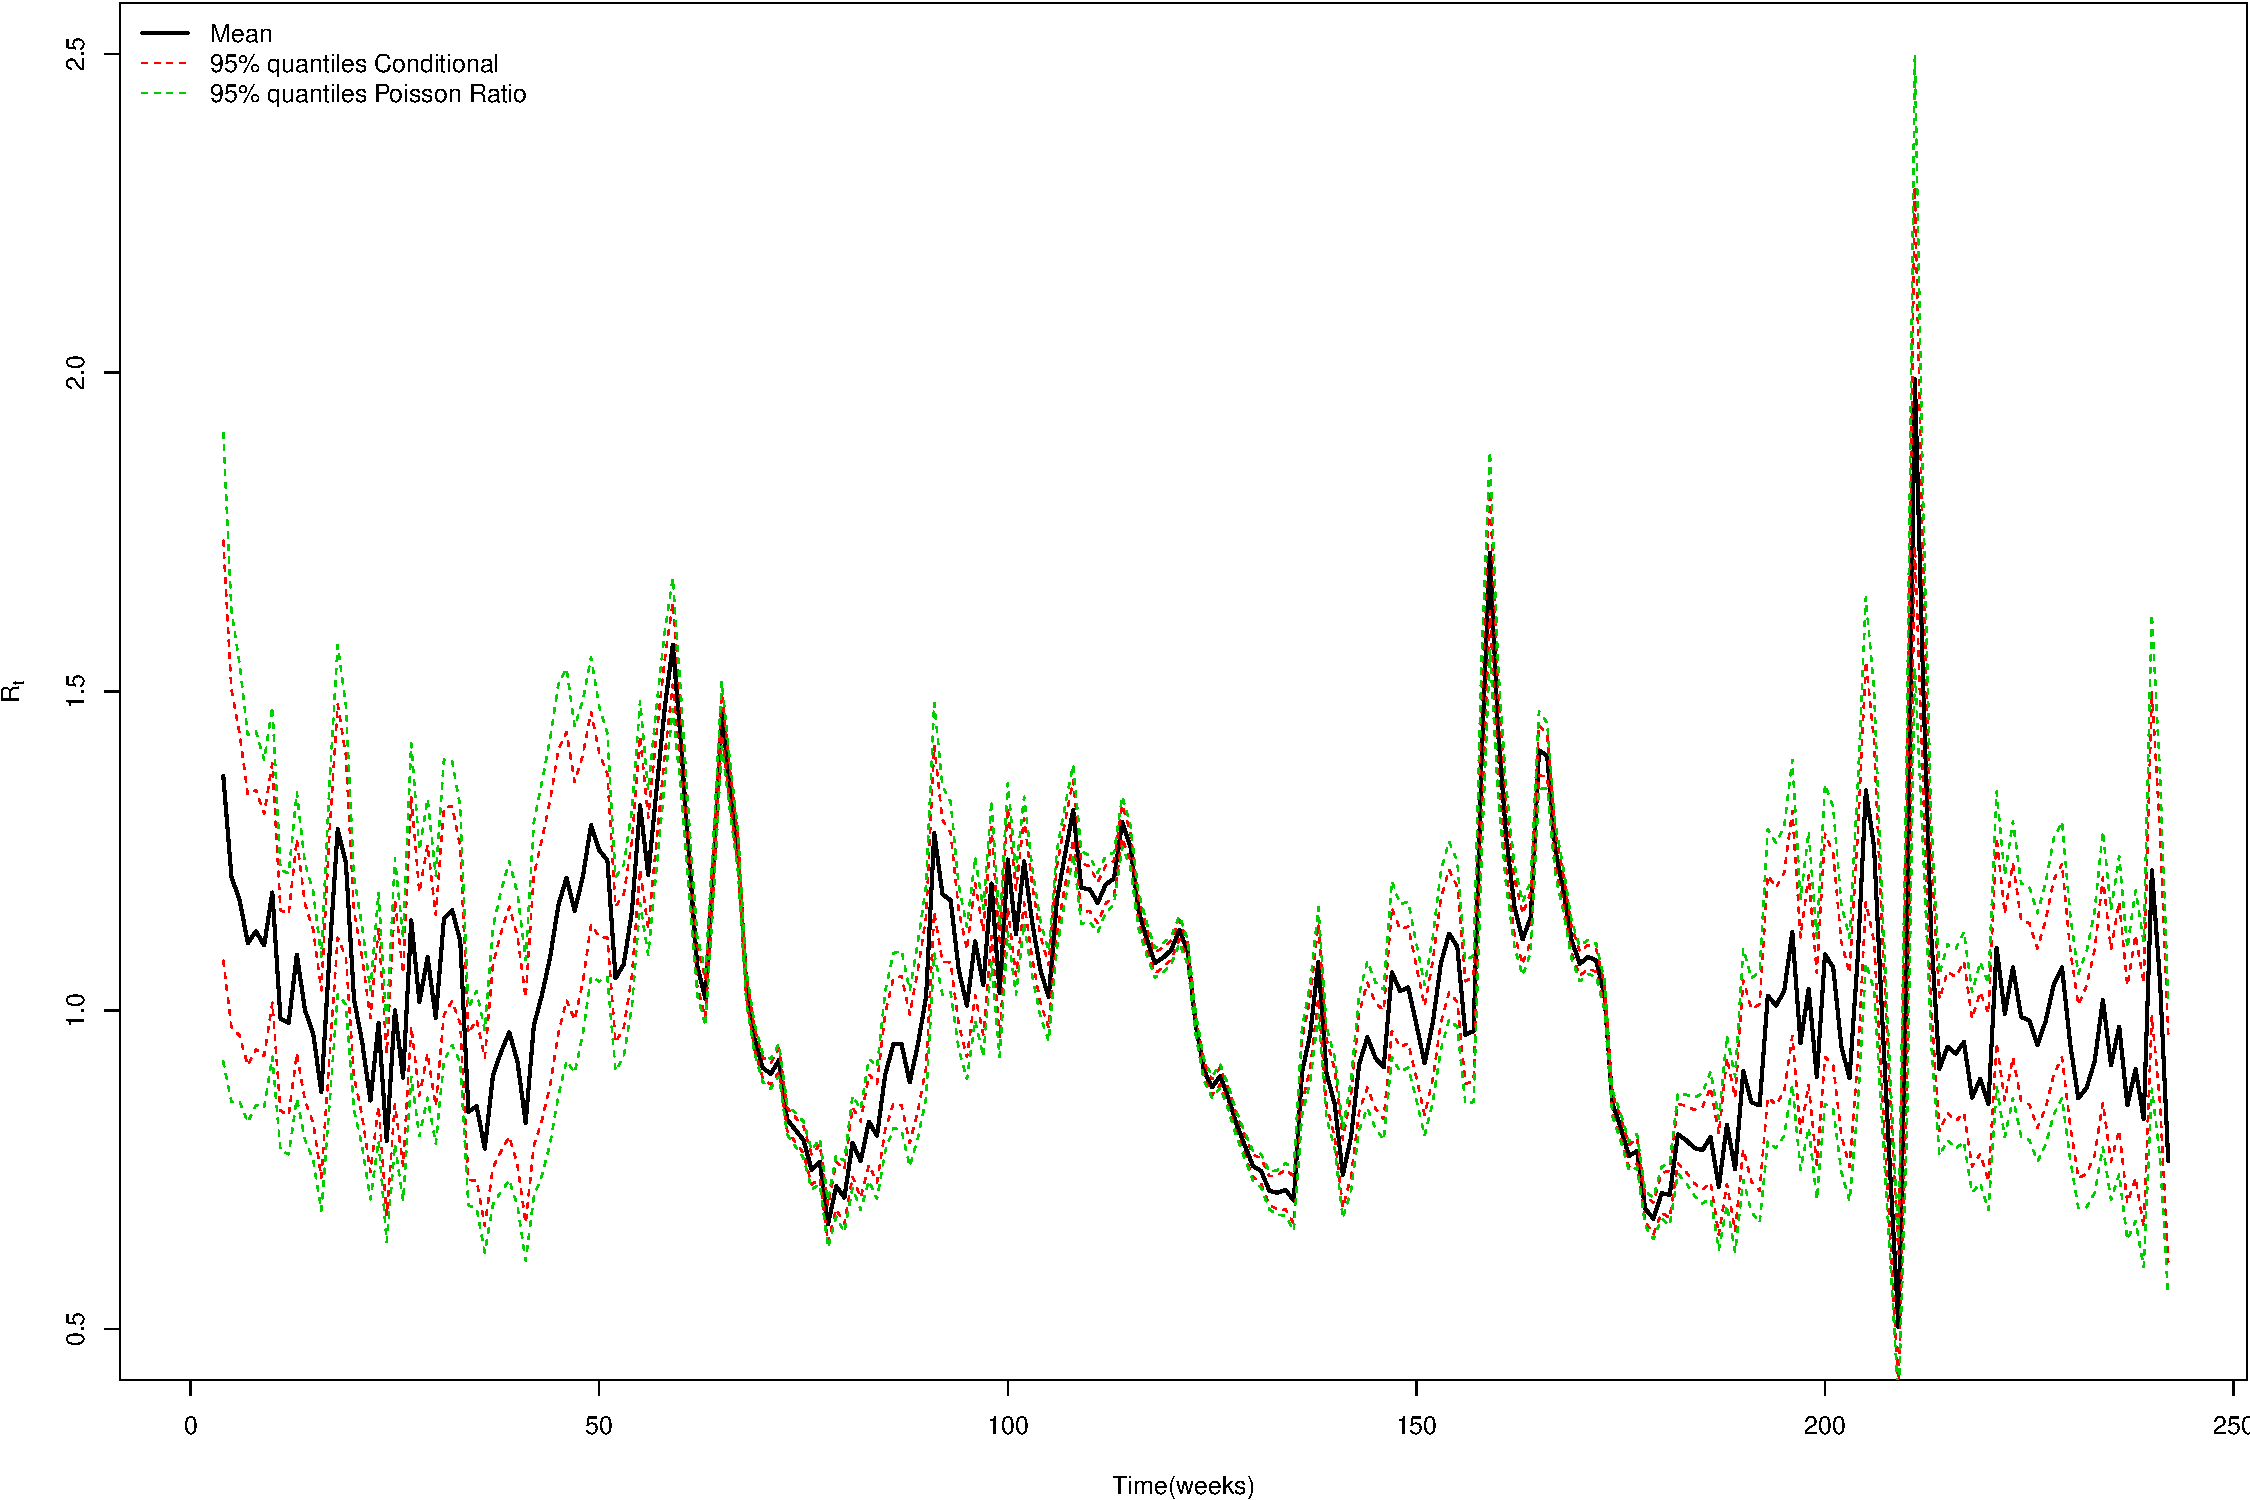
\includegraphics{FIGURES/figure-003}
\end{center}
\caption{\rr estimates for the total notifications and confidence intervals obtained using the two proposed methods.}
\label{fig:confidencetotals}
\end{figure}
%%%%%%%%%%%%%%%%%%%%%%%%%%%%%%%%%%%%%%%%%%%%%%%%%%%%%%%%%%
\begin{figure}[!h]
\setkeys{Gin}{scale=.7}
\begin{center}
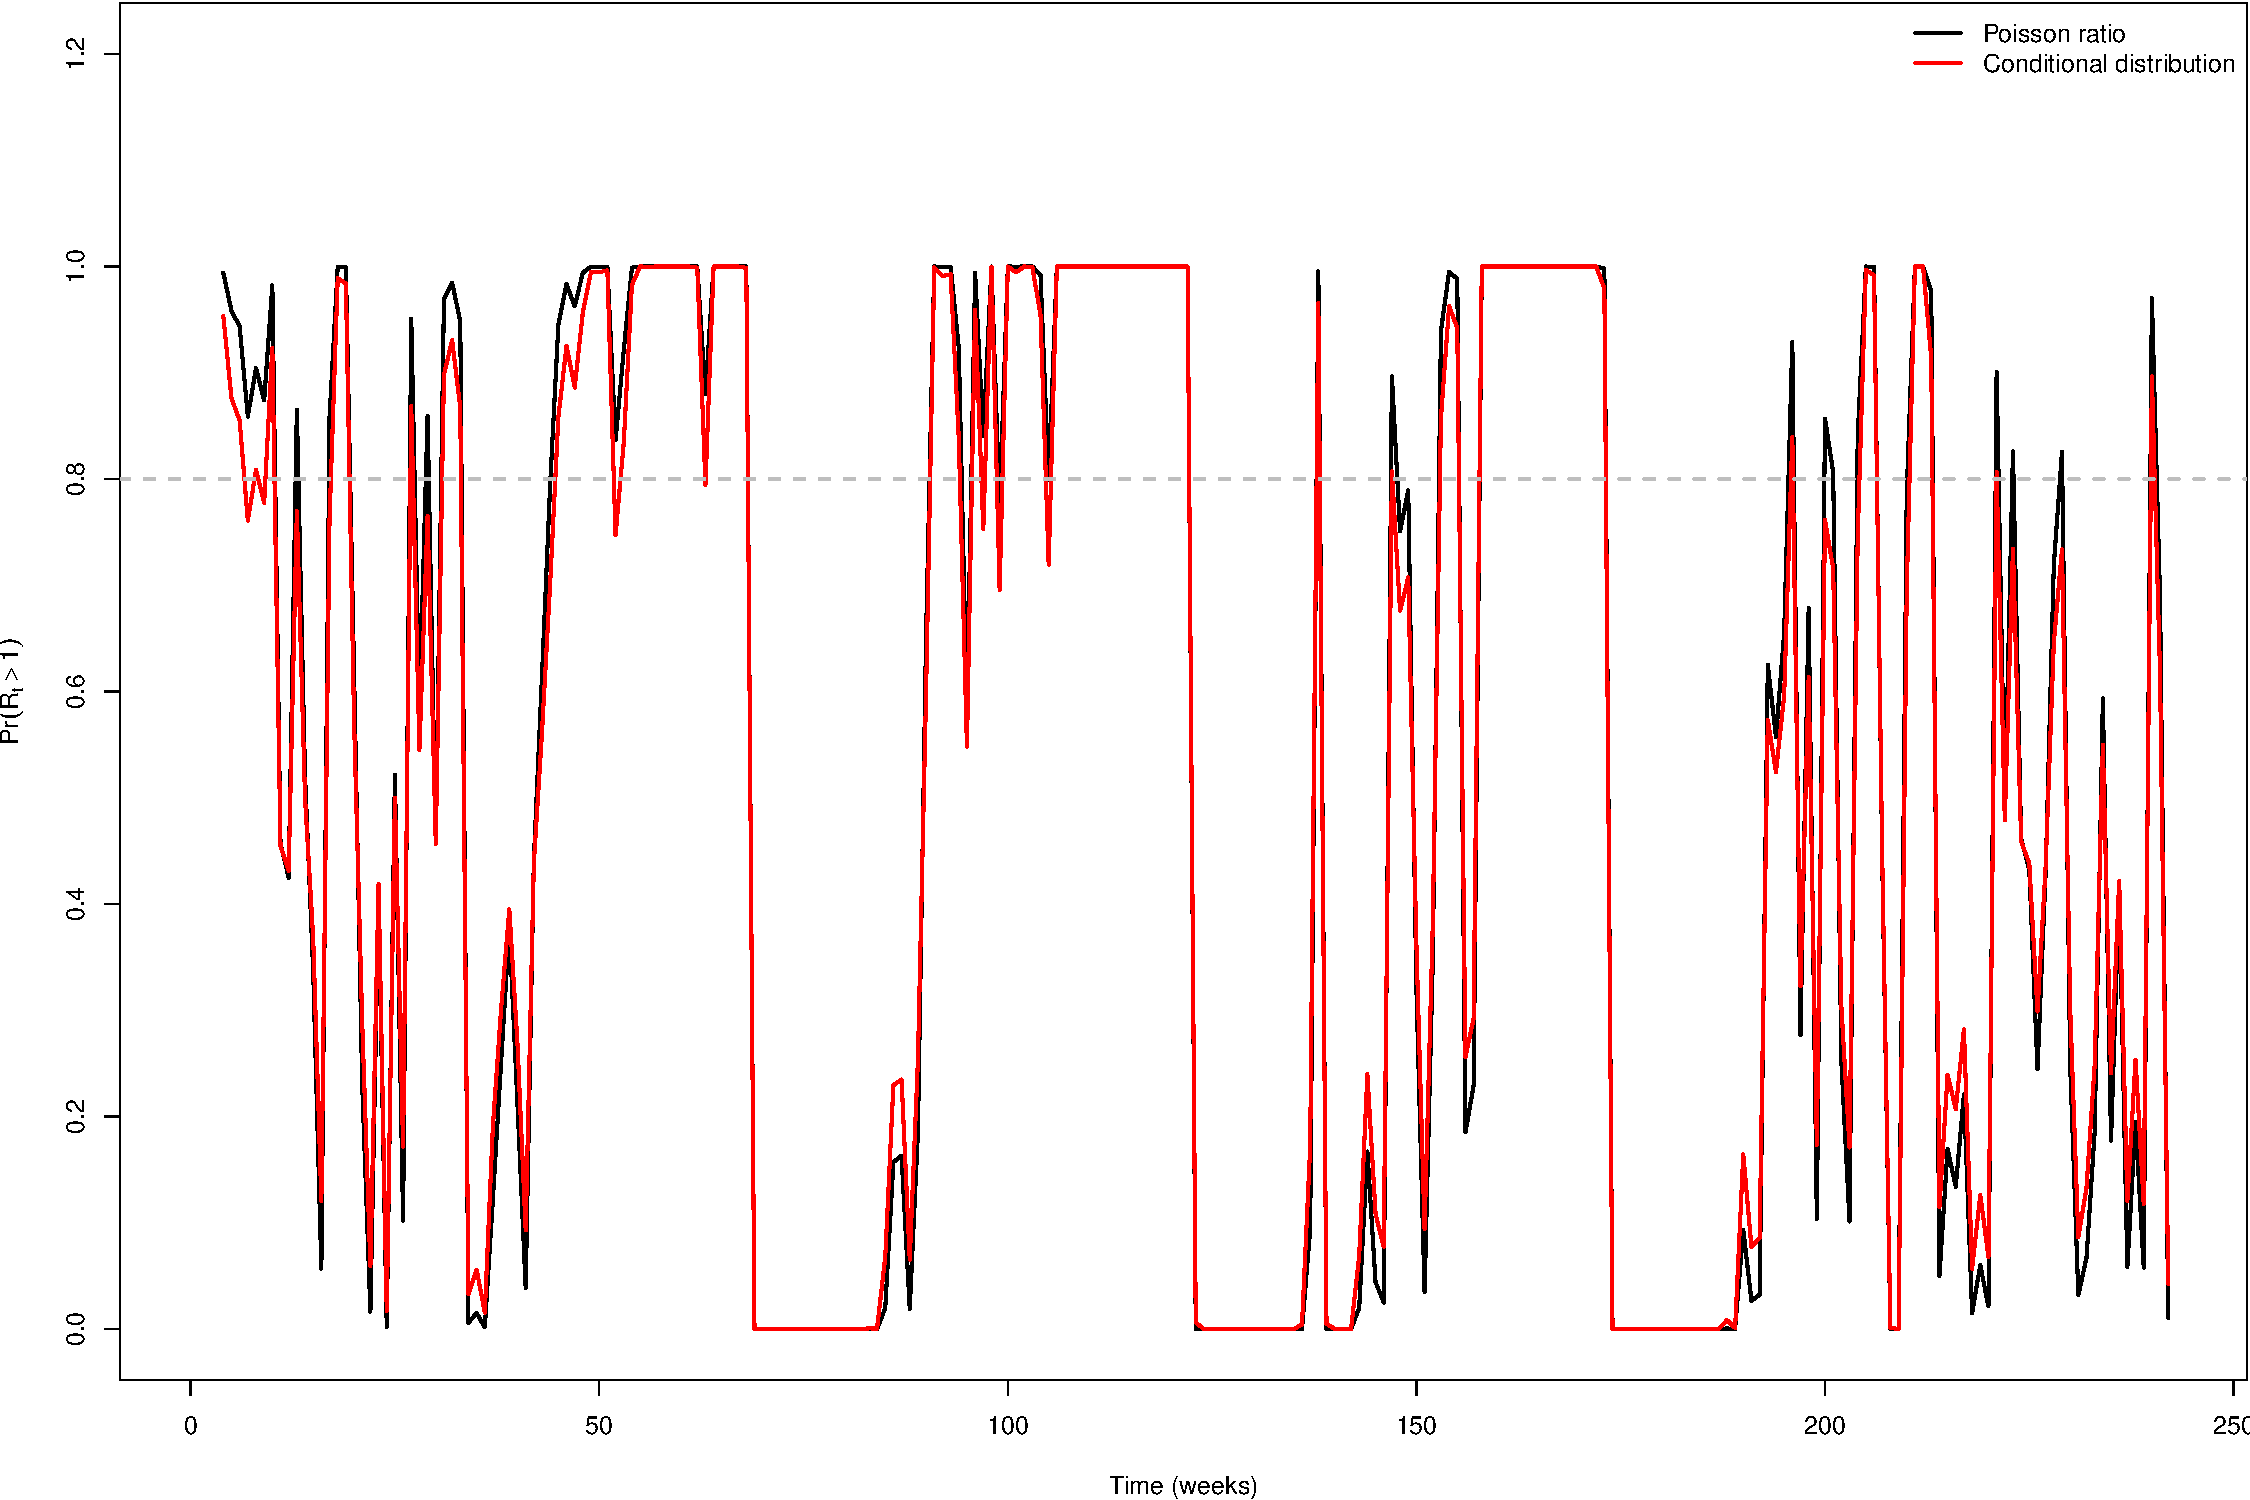
\includegraphics{FIGURES/figure-004}
\end{center}
\caption{Probability that $R_t \geq 1$.
The interrupted gray line marks the arbitrary value of $0.80$.  
}
\label{fig:pRt1}
\end{figure}
%%%%%%%%%%%%%%%%%%%%%%%%%%%%%%%%%%%%%%%%%%%%%%%%%%%%%%%%%
\newpage
\bibliography{lm1}
\end{document}
